\section{Background}%
\label{sec:background}
This section provides an overview of the research that underlies the main results
of this thesis, with a focus on \emph{program analysis}. Specifically, we will delve into
the concepts of dataflow analysis~\cite{aho2007compilers,Nielson2010Principles},
control-flow analysis~\cite{allen1970control}, (Reference) attribute grammars~\cite{knuth1968semantics,hedin2000rags},
and their implementation through the \textsc{JastAdd} metacompiler.

\usetikzlibrary{backgrounds}
\begin{figure}[h]
    \centering
    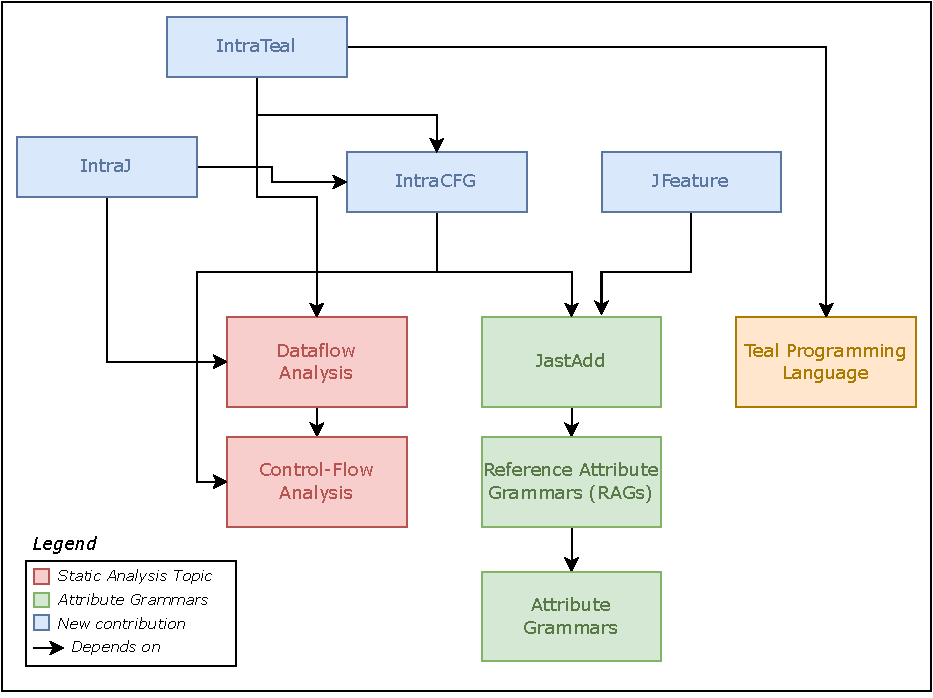
\includegraphics[width=0.9\textwidth]{kappa/img/Dependencies.pdf}
  \caption{\label{fig:dependencygraph}Dependency graph of the concepts discussed in this Section.}
\end{figure}
The dependency graph in Figure~\ref{fig:dependencygraph} shows the relationship between
the concepts and the contributions of this thesis.

\subsection{Automatic Program Analysis}
Automatic Program Analysis is a branch of computer science that aims to automatically
analyse and evaluate programs' properties, e.g., \emph{correctness}, \emph{liveness} and \emph{safety}. We can distinguish two main
approaches to program analysis: \emph{static} and \emph{dynamic} analysis.

Dynamic analysis examines the behaviour of a program by executing it.
Precise information about a single program's execution are gathered
and used to determine the properties of the program.
This approach is effective in detecting runtime errors, such as memory leaks~\cite{Valgrind},
performance bottlenecks~\cite{Intel}, and security vulnerabilities~\cite{li2018fuzzing}.
However, its limitations come from the requirement for complete and
accurate input data for a single run, and the difficulty in accounting for
all possible execution paths.

In contrast, static analysis performs the analysis without executing the program,
relying on information gathered from the source code. This approach has
the advantage of being more exhaustive, as it can analyse the entire program.
One limitation of static analysis is that it can result in \emph{false positive}
and \emph{false negative} results. False positive results occur when the analysis
incorrectly reports a problem in the code, whereas false negative results occur
when the analysis fails to report an actual problem in the code. The \emph{soundness} and
\emph{completeness} of the analysis determine the accuracy of the results. Soundness refers
to the property that if the analysis reports a problem, then there is indeed a
problem in the code.
Completeness refers to the property that if there is a problem
in the code, the analysis will eventually report it. In practice, it is often
difficult to achieve both soundness and completeness, which leads to the trade-off
between false positive and false negative results in static analysis.

Important kinds of static analysis include  \emph{Type}
and \emph{Effect analyses}~\cite{nielson1999type}.
Type Analysis aims to determine the type of variables and expressions
in a program, which can be used to identify type mismatches, type errors, and improve
code readability. Effect analysis focuses on the study of side effects that a program can
produce, such as the mutation of data. This information can be used to identify
potential bugs and improve program understandability.

In this thesis, we focus on intraprocedural control-flow and dataflow analysis,
that are crucial for implementing many type and effect analyses.
Intraprocedural control-flow analysis focuses on determining the order in which
statements and expressions within a single method in a program will be executed,
without considering any function or method calls that may occur.
Intraprocedural dataflow analysis uses the control-flow information to
determine properties on the flow of data within a single method.
Our implementations are instances of the Monotone Framework, a mathematical framework that provides a
foundation for dataflow analysis. In the future, we aim to improve the precision of the analysis
by considering the implementation of interprocedural analysis, which involves
analysing the flow of data across multiple procedures in a program.

Precision is a crucial aspect of dataflow analysis.
Depending on the desired outcome, various levels of precision can be achieved,
but it is important to weigh the trade-off between precision and performance.
A higher level of precision often requires increased computational resources,
leading to a decrease in performance, and vice versa. Hence, finding the right
balance between precision and performance is crucial in achieving effective and
efficient dataflow analysis results.

In our research, we have chosen to compute control-sensitive and
exception-sensitive control-flow analyses.
Control-sensitivity refers to the ability of the analysis to distinguish between
true and false branches of conditional statements, such as if-statements, and
taking into account the implicit side effects of the conditional expressions.
Exception-sensitivity refers to the ability of the analysis to distinguish between
the normal and exceptional execution paths of a program.
This approach simplifies the specification of dataflow analyses which are built upon the
control-flow analysis.

In terms of implementation strategies, there are various approaches that can be
used, including Datalog~\cite{dura2021javadl}, functional programming~\cite{madsen2016datalog}, or ad-hoc implementation.
However, we choose to implement the analysis using Reference Attribute Grammars~\cite{hedin2000rags}.
This approach allows us to exploit the benefits of modularity, high-level programming,
and on-demand evaluation, which results in a flexible and efficient implementation.

We recognise that the results of our analyses, while effective,
may not be sound nor complete and that the analysis may not be able to identify
all the bugs or vulnerabilities in a program~\cite{livshits2015defense}.





\subsection{Control-flow analysis}
Control-flow analysis refers to the computation of
 the execution and evaluation order of the program's statements and expressions.
Each possible execution order of a program is called a control-flow path.
The result of the control-flow analysis is a control-flow graph (CFG) $G=(V,E)$.
Each vertex $v \in V$ represents a unit of execution, e.g., a single statement or expression,
or a basic block (a sequence of statements without labels and jumps).
Each edge $(v_1,v_2) \in E$  represents a control-flow edge, indicating that the
execution of $v_1$ may be directly followed by the execution of $v_2$.

We can distinguish two main approaches to constructing the CFG for a program:
on the source level and the intermediate representation (IR). The source-level approach
involves analysing the source code of a program and constructing the CFG
directly from the source code on top of the abstract syntax tree. The IR approach involves
first converting the source code into an IR, e.g., bytecode,
and then constructing the CFG from the IR.%

The construction of the CFG at the source level presents several advantages. One of the
main benefits is the ability to map the analysis results directly back to the source code
and present it to the user in the context of the original program. On the other hand,
if the CFG is constructed at the IR level, there would be a complex translation step
required to find the corresponding source level constructs. In some cases it would
not even be possible due to the loss of information during the translation process, e.g.,
\code{source-file retention} policy for Java annotations.
For this reason, constructing the CFG at the source level is particularly useful for
debugging and program understanding tasks, as it provides a clear and direct
representation of the program. Additionally, this approach enables faster and
more efficient analysis as it eliminates the overhead of IR generation and can
also handle semantically and syntactically invalid code, making it useful for
analysing programs with errors or incomplete code. Furthermore, in situations where
IR generation must occur in real-time, such as when the analysis is performed in an
IDE, the overhead of code generation and optimisation may cause latency in the IDE and frustration for the developer~\cite{piskachev2022far}.
In these cases, constructing the CFG at the source level may be a more efficient option.

However, there are also some disadvantages to constructing the CFG on the source level.
One of the main limitations is that it can be more difficult to accurately capture the
control-flow of a program since the source code may contain unsugared constructs,
such as macros and preprocessor directives, that
can complicate the analysis specification.
In comparison to the engineering effort required by the IR approach, the source-level
approach presents complex implementation challenges. Despite the advantage
of IRs being generally smaller than the source language, thus reducing the number
of constructs to be handled in constructing the CFG and potentially reducing
the size or complexity of the analysis code, the source-level approach requires
a higher level of complexity in its implementation.
In addition, the source code may be written in a variety
of languages with different syntax and semantics, making it challenging to
design a single analysis that works across all languages.

The examples in Figures~\ref{fig:cfgsourcelevel} and~\ref{fig:cfgintermediatelevel} show the source-level and bytecode control-flow
graphs of a simple method \texttt{foo}.
Adding \emph{Entry} and \emph{Exit} nodes to a CFG is a common practice to
simplify the implementation of dataflow analyses.
These nodes represent the unique entry and exit points of the method, respectively.
The Entry node serves as a starting point for the
analysis, allowing for a proper initialisation of the parameters.
The Exit node is particularly useful in backward dataflow analyses (see Section~\ref{sec:dataflowanalysis}), as it is used
as unique starting point for the analysis.
\begin{figure}[H]
  \centering
\begin{tabular}{l r}
  \begin{lstlisting}[language=JastAdd]
void foo(boolean b){
  Integer x = 0;
  if (b) {
    x = 1;
  } else {
    x = null;
  }
}
  \end{lstlisting} &\hspace{2.5cm}
  \begin{tikzpicture}[node distance=1.35cm, baseline=(current bounding box.center)]
      \node (start) [rectangle] {\texttt{Entry}};
      \node (assign) [rectangle, below of=start] {\texttt{x = 0}};
      \node (if) [rectangle, below of=assign] {\texttt{if (b)}};
      \node (then) [rectangle, below of=if] {\texttt{x = 1}};
      \node (else) [rectangle, right = 0.3cm of then] {\texttt{x = null}};
      \node (end) [rectangle, below of=else] {\texttt{Exit}};
      \draw [->] (start) -- (assign);
        \draw [->] (assign) -- (if);
      \draw [->] (if) -- node [left, font=\scriptsize] {\textsc{true}} (then);
      \draw [->] (if) -- node [right,  font=\scriptsize]{\textsc{false}} (else);
      \draw [->] (then) -- (end);
      \draw [->] (else) -- (end);
  \end{tikzpicture}
  \end{tabular}
  \caption{\label{fig:cfgsourcelevel}Source level control-flow graph of the \texttt{foo} method, showing the branching behaviour of the \code{if}-statement.}
\end{figure}


\begin{figure}[H]
  \centering
\begin{tabular}{l r}

\begin{lstlisting}[language=bytecode, frame=none]
    1 :0 : iconst_0
    2 :1 : invokestatic  #7
    3 :4 : astore_2
    4 :5 : iload_1
    5 :6 : ifeq          17
    6 :9 : iconst_1
    7 :10: invokestatic  #7
    8 :13: astore_2
    9 :14: goto          19
    10:17: aconst_null
    11:18: astore_2
    12:19: return
\end{lstlisting}
&\hspace{2.5cm}
\scalebox{0.85}{
\begin{tikzpicture}[
  node distance=0.25cm,
  every node/.style={shape=rectangle, align=center},
  baseline=(current bounding box.center)]
  % Nodes
  \node (1) {1};
  \node (2) [below=of 1] {2};
  \node (3) [below=of 2] {3};
  \node (4) [below=of 3] {4};
  \node (5) [below=of 4] {5};
  \node (6) [left=of 5] {6};
  \node (7) [below=of 6] {7};
  \node (8) [below=of 7] {8};
  \node (9) [below=of 8] {9};
  \node (10) [right=of 5] {10};
  \node (11) [below=of 10] {11};
  \node (14) [below=of 5] {};
  \node (15) [below=of 14] {};
  \node (16) [below=of 15] {};
  \node (12) [right=of 9] {12};
  \node (exit) [right=of 12] {\texttt{exit}};
  \node (entry) [left=of 1] {\texttt{entry}};

  % Edges

  \path[-stealth] (1) edge (2);
  \path[-stealth] (2) edge (3);
  \path[-stealth] (3) edge (4);
  \path[-stealth] (4) edge (5);
  \path[-stealth] (5) edge[bend right] (6);
  \path[-stealth] (5) edge[bend left] (10);
  \path[-stealth] (6) edge (7);
  \path[-stealth] (7) edge (8);
  \path[-stealth] (8) edge (9);
  \path[-stealth] (9) edge (12);
  \path[-stealth] (10) edge (11);
  \path[-stealth] (11) edge (12);
  \path[-stealth] (12) edge (exit) (entry) edge (1);
  \draw[dashed] (1.north west) rectangle (2.south east);
  \draw[dashed] (3.north west) rectangle (5.south east);
  \draw[dashed] (6.north west) rectangle (7.south east);
  \draw[dashed] (8.north west) rectangle (9.south east);
  \draw[dashed] (10.north west) rectangle (11.south east);
  \draw[dashed] (12.north west) rectangle (12.south east);
\end{tikzpicture}}
\end{tabular}
\caption{\label{fig:cfgintermediatelevel}Bytecode control-flow graph of the \texttt{foo} method. Each dashed box represents a basic block.}
\end{figure}




\subsection{Dataflow Analysis}%
\label{sec:dataflowanalysis}
Dataflow analysis is a technique used to analyse the flow of
data through a program. It has its roots in the field of program optimisation~\cite{kildall1973dataflow},
where it was initially used to identify opportunities for improving the performance
of programs by tracking variable definitions and uses. This information can be used to optimise the program by eliminating
unnecessary computations (e.g., Very Busy Expression or Available Expression
analyses~\cite{aho2007compilers}) and improving
the use of available resources (e.g., registers optimisation).


In the context of bug detection, dataflow analysis can be used to identify
potential sources of errors in a program by tracking the flow of data through
the program and identifying points where data may be used in unexpected or
incorrect ways. This can be particularly useful in identifying bugs that may
not be immediately apparent, such as those that only occur under certain
conditions or when certain combinations of input data are used (e.g., \texttt{IndexOutOfBound} exception).
Many static analysis tools for Java programs, e.g., FindBugs, employ intraprocedural
dataflow analysis to identify potential bugs in Java code.
% I looked here how they cited pmd, findbugs and spotbugs. https://ieeexplore.ieee.org/stamp/stamp.jsp?tp=&arnumber=8103456
Dataflow analysis, particularly interprocedural dataflow analysis, is widely
used to identify potential security vulnerabilities in software~\cite{flowDroid}.
For example, an interprocedural control-flow graph enables tracking of the flow
across multiple methods or functions, thereby allowing identification of points
where the data may be exposed to unauthorized access or manipulation.

We will demonstrate an application of intraprocedural dataflow analysis by presenting the following
practical, but incomplete, example. Let us reconsider the \code{foo} method introduced in Figure~\ref{fig:cfgsourcelevel}.
Our goal is to determine at each stage of the program whether the variable \code{x}
has a \code{null} value or not\footnote{For simplicity, just for this example, we assume that the language
allows only assignments of the form \code{x = y} where \code{y} can
be either a  variable, a numeric constant or the \code{null} literal. We also assume
that CFG nodes are individual assignments.
}.

At the entry point of the method, i.e., Entry node,
it is indeterminate whether \code{x} is \code{null} or not, as it has not been initialized yet.
However, at the declaration of the variable \code{x}, we can determine that it is
not \code{null} because it is initialised to a non-\code{null}
value. Then, if the condition \code{if(b)} is \code{true}, the
variable \code{x} is assigned a new value, which is not \code{null}. If the condition
is \code{false}, the variable \code{x} is assigned \code{null}. Therefore, at the
end of the method, the variable \code{x} may be either \code{null} or not \code{null}.
Consider the scenario where \code{x} is used and dereferenced immediately after the
if-else statement, for example, calling a method on \code{x}. The program will then crash,
with a \code{NullPointerException}, if \code{x} is \code{null}.
Dataflow information can be used to identify potential bugs like this in a program.

We keep track of the value of \code{x} by mapping it to a finite set of possible values:
\code{null}, \code{notnull}, \code{maybenull}, or \code{unknown}.
As we traverse the control-flow graph, we propagate this information from node
$n$ to node $n'$ if $(n,n')\in E$, until it reaches the Exit node.

The information is updated at each node $n$ according to the following rules:
\begin{itemize}
\item If $n$ is an assignment node, the information is updated according to the
assignment operation. For example, if the assignment is \code{x = null}, then
it is recorded that \code{x} is updated to \code{null}. If the assignment is \code{x = y}, then
\code{x} is mapped to the value \code{y} maps to.
\item If $n$ is not an assignment node, no information is updated.
\end{itemize}

The dataflow analysis just described is an instance of the mathematical concept of
Monotone Frameworks~\cite{Nielson2010Principles}.

\subsubsection*{Monotone Frameworks}
\label{sec:monotoneframeworks}
Monotone frameworks are a theoretical approach for reasoning
about program dataflow properties.
This approach provides a flexible and generic framework for expressing and solving
dataflow equations, which can be used to reason about a wide range of dataflow
properties, such as \emph{live variables}, \emph{reaching definitions} and \emph{available expressions} analyses.
Monotone frameworks are built on the concept of lattices~\cite{Donnellan1968}.

A lattice $\mathcal{L} = (S, \leq)$ is a partially ordered set in which any two elements have a unique least
upper bound (also known as a join or a supremum) and a unique greatest lower bound
(also known as a meet or an infimum). This means that, for any elements $a$ and $b$ in
$S$, there exists a unique element denoted as  $a \sqcup b$  (or  $a \vee b$)
such that  $a \leq a \sqcup b$  and  $ b \leq a \sqcup b$, and  $a \sqcap b$
(or  $ a\wedge b$) such that  $ a\sqcap b\leq a$  and  $a \sqcap b\leq b$.
A complete lattice has a unique least element, commonly denoted as $\bot$,
and a unique greatest element commonly denoted as $\top$. These elements satisfy
the properties that for any element $x$ in the lattice, $\bot \leq x$ and $x \leq \top$.
In dataflow analysis, lattices are widely used to represent the information flow in a program.
A common example of a lattice used in dataflow analysis is the \emph{binary lattice} with
elements \emph{true} and \emph{false}, which is used to represent the presence or absence of
a property. Another example is the \emph{interval lattice}, which is used
to represent ranges of numbers. This lattice, compared to the binary lattice, is more
complex but provides more precise information about the flow of numerical values
in a program. Additionally, while the binary lattice is \emph{finite} height, the interval lattice can
be potentially \emph{infinite}.
\begin{wrapfigure}{r}{0.5\textwidth}
     \begin{center}
  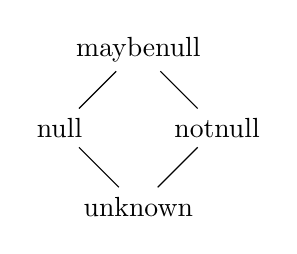
\begin{tikzpicture}
      \node (top) at (0,1) {\code{maybenull}};
      \node (null) at (-1,0) {\code{null}};
      \node (notnull) at (1,0) {\code{notnull}};
      \node (bot) at (0,-1) {\code{unknown}};
      \draw (bot) -- (null) -- (top) -- (notnull) -- (bot);
    \end{tikzpicture}
    \caption{\label{fig:lattice}Diagram of the partial order in the example in
    Section~\ref{sec:dataflowanalysis}, showing the order relation between \code{maybenull}
    ($\top$), \code{unknown} ($\bot$), \code{null}, and \code{notnull}.}
  \end{center}
\end{wrapfigure}


Monotone frameworks include a join operator $\sqcup$, a monotone transfer function $f$,
and a finite height lattice $\mathcal{L}$.
A monotone transfer function is a mathematical function that maps an element of a
partially ordered set to another element in the same set such that the partial
ordering is preserved under the function. More formally, if $(S, \leq)$ is a
partially ordered set and $f: S \rightarrow S$ is a function, $f$ is called a
monotone transfer function iff, for all $x, y \in S$ such that $x \leq y$, it follows
that $f(x) \leq f(y)$.

In our example, the lattice $\mathcal{L}$ is used to model the possible values,
i.e., \code{null}, \code{notnull}, \code{maybenull}, and \code{unknown}, that a variable can assume.
This lattice is shown in Figure~\ref{fig:lattice}. Here \code{maybenull} is
the greatest element in the lattice, as it represents the set of all possible values
that a variable can take. On the other hand, \code{undefined} is the least element
representing the absence of information.
The join operator $\sqcup$ merges the information of two nodes. For instance, if node $n$ has information \code{null} and node $n'$ has
information \code{notnull}, then the information at the merged node $n \bigsqcup n'$
becomes \code{maybenull}.
In the previous section, we explained how a node affects the flow of data
using natural language. Now, we will present this concept in a formal manner
as a transfer function. Let \textit{Var} be the set of variables in the program,
$V$ be the set of nodes in the CFG, and  $\Gamma:\textit{Var} \rightarrow \mathcal{L}$
be the function that maps variables to elements of the lattice $\mathcal{L}$.
The monotone transfer function $f_{\textit{NULL}}: (\textit{Var} \rightarrow \mathcal{L}) \times V \rightarrow (\textit{Var} \rightarrow \mathcal{L})$
is defined as follows:

\[
  f_{\textit{NULL}}(\Gamma, \vterminal{node}) =
  \begin{cases*}
  \Gamma[\vmetavar{v} \mapsto \semNPA{\vmetavar{e}}^\Gamma] & if  \vterminal{node} is \vterminal{\vmetavar{v} = \vmetavar{e}}  \\
  \Gamma  & otherwise
\end{cases*} \]%

\[
\begin{array}{llcl}
\textrm{where}&\semNPA{\vterminal{n}}^\Gamma  \text{ for } \vmetavar{n}\in \textit{Num}			&=& \textbf{notnull}\\
&\semNPA{\vterminal{null}}^\Gamma			&=& \textbf{null}\\
&\semNPA{\vmetavar{v}}^\Gamma \text{ for } \vmetavar{v}\in \textit{Var}				&=& \Gamma(\vmetavar{v}) \\
\end{array}
\]


To propagate information from node $n$ to its succeeding nodes (in the CFG) and to represent the
effect of passing through a node, we define the following two equations:
\begin{align*}
  \text{in}(n) &= \begin{cases} \{ v \rightarrow \bot \mid \forall v \in $\textit{Var}$ \} & $if $ n $ is Entry$ \\ \bigsqcup\limits_{p \in \text{pred}(n)} \text{out}(p) & $otherwise$ \end{cases} \\
  \text{out}(n) &= f_{\text{\textit{NULL}}}(\text{in}(n),n)
\end{align*}
where $\text{pred}(n)$ is the set of predecessor of the node $n$, i.e., $\text{pred}(n) = \{ p \mid (p,n)\in E\}$ and $E$ is the set of edges in the CFG.
We have defined the $in$ and the $out$ sets to model the information that is available
before and after passing through a node, respectively. The $in$ set gathers the available
information before entering the node, while the $out$ set captures the effect
of applying the transfer function $f_{\textit{NULL}}$ on the $in$ set.
This kind of analysis is called a \emph{forward analysis} because it propagates information
from the entry node to the exit node.

These equations can be adapted to perform backward analyses, i.e., analyses that
propagate information from the exit node to the entry node. Let us look at the
general definition of a backward analysis.
Given a monotonic transfer function $f$ and a finite lattice $\mathcal{L}$, the equations for
a backward analysis is defined as follow:
\begin{align*}
  \text{out}(n) &= \bigsqcup\limits_{s \in \text{succ}(n)} \text{in}(s) \\
  \text{in}(n) &= f(\text{out}(n),n)
\end{align*}
where $\text{succ}(n)$ is the set of successors of the node $n$, i.e., $\text{succ}(n) = \{ s \mid (n,s)\in E\}$.
The boundary condition for the $\textit{out}$ set when $n$ is the Exit node differs depending on the
analysis.

The equations for both forward and backward analyses define a mutual dependency
between the $in$ and $out$ sets of a node.
A fixpoint computation is used to resolve this circular dependency. A fixpoint is
a mathematical technique that finds a stable state, in a system.
In the context of the Monotone frameworks, this
refers to finding a state where the $in$ and $out$ sets of all nodes in the CFG have reached a
stable value, and no further changes will occur. The authors of~\cite{Nielson2010Principles}
present several techniques for computing fixpoints. They demonstrate that there exists a fixpoint~\cite{Knaster1929} and that the resulting
fixpoint is the unique and the minimum among all fixed points of the transfer function $f$.




\subsection{Attribute Grammars}%
\label{chap:attr-grammars}
Attribute grammars~\cite{knuth1968semantics} (AGs) are a formalism for specifying
the syntax and semantics of programming languages. This formalism is based on the concept of attributes,
which are properties associated with the elements of a language's abstract syntax tree.
Attribute grammars provide a powerful tool for specifying the behaviour of a programming
language and for verifying compile-time correctness of programs written in that language.
%
AGs are composed of three components: a context-free grammar,
which defines the language's syntax,  a set of attributes,
which are properties associated with the nodes of the abstract syntax tree,
and attribute equations, used to compute the values of the attributes associated
with each node in the abstract syntax tree.

Attribute grammars enable the description of the
interdependence of syntactic and semantic elements of a programming language.
For instance, the type of a variable may be determined by its declaration,
but the type of an expression may be determined by the types of its sub-expressions.
Attribute grammars provide a way to specify these rules.

We can distinguish two types of attributes: synthesized attributes and inherited attributes.
For the sake of readability, we use the notation introduced by Fors et al. in~\cite{fors2020patterns},
where attribute names are preceded by a symbol (e.g.,\textcolor{ATGsym}{\mSyn{}},\textcolor{ATGsym}{\mInh{}})
that indicates the kind of the attribute (e.g., synthesized or inherited).

A \emph{synthesized} attribute is a property of a node that is computed
based on the attributes of the subtree rooted at that node. For example, the type of an expression
in a programming language may be a synthesized attribute computed based
on the types of sub-expressions in the expression. For instance, the type of the expression ``3 + 4'',
is determined to be integer based on the types of the operands.

Synthesized attributes are composed by a declaration and an equation:
\begin{align*}
  \astnode{T}\ &\Asyn{A}{x} \\
   &\Asyn{A}{x} = e
\end{align*}
where \astnode{T} is the type of the attribute, \astnode{A} is the node type, and \textcolor{ATGsym}{x} is the attribute name.
The up-arrow symbol (\textcolor{ATGsym}{\mSyn{}}) is used to denote a synthesized attribute.
The right-hand side of the equation, is an expression, $e$, that may use other attributes of the \astnode{A} node or its children.
If \astnode{A} has subtypes, say \astnode{A1}$<:$\astnode{A} and \astnode{A2}$\l<:$\astnode{A}, different equations can be given for
\astnode{A2} and \astnode{A1}. If all subtypes will use the same equation, the declaration and the equation can be combined into a single line, as follows:
\begin{equation*}
 \astnode{T} \  \Asyn{A}{x} = e
\end{equation*}

% We use the symbol \Abase{x} to denote the attribute name and the symbol $e$ to denote the attribute value,
% e.g., a constant, or a function of the node's children and/or the node's own attributes.

An \emph{inherited} attribute is a property of a node that gets its value from
its parent in the abstract syntax tree.
An example of inherited attribute is the expected type of an expression.
The expected type of an expression is inherited from the context in which the expression is used.
For example, the expected type of the condition in an \code{if}-statement is boolean.
This information is inherited from the \code{if} statement node.

Inherited attributes are defined in two parts: a declaration and an equation.
\begin{align*}
 \astnode{T} \ &\Ainh{B}{x} \\
 &\Ainhdef{A}{B}{x} = e
\end{align*}
where \astnode{A} and \astnode{B} are node types and the down-arrow symbol (\textcolor{ATGsym}{\mInh{}}) is used to denote an inherited attribute.
The equation defines the \textcolor{ATGsym}{x} attribute of \astnode{A}'s child \astnode{B}.
The expression $e$ may use the attributes of \astnode{A} and any of its children.


\begin{figure}
\centering
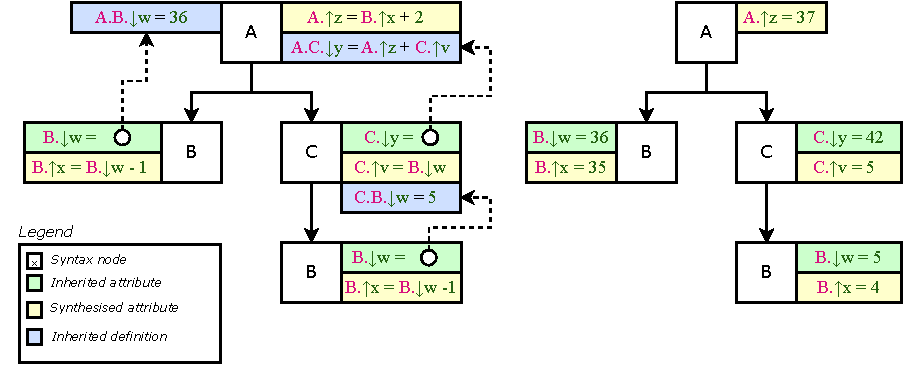
\includegraphics[width=1\textwidth]{kappa/img/AGExample.pdf}
    \caption{\label{fig:ragsExample} Attribute grammar example.
    Left: Abstract syntax tree with attribute equation system. Right: solution of the equation system.
    Dashed arrows indicates the location of the equation for an inherited attribute.
    }
\end{figure}

To better explain the concept of AGs, we present a very simple example.
We start by defining the following abstract grammar:
    \begin{align*}
        A& ::= B \quad C \\
        B& \\
        C& ::= B
    \end{align*}
and the following attribute declarations and equations:
    \begin{align*}
        &\textit{Synthesized:}  && \textit{Inherited:} \\
        &\nativetype{int} \ \Asyn{A}{z} = \Asyn{B}{x} + 2  &&\nativetype{int} \ \Ainh{C}{y} \\
        &\nativetype{int} \ \Asyn{B}{x} = \Ainh{B}{w} -1   &&\nativetype{int} \ \Ainh{B}{w}  \\
       &\nativetype{int} \ \Asyn{C}{v} = \Ainh{B}{w}   & &\Ainhdef{A}{B}{w} = 36\\
        & && \Ainhdef{C}{B}{w} = 5\\
        &&& \Ainhdef{A}{C}{y} = \Asyn{A}{z} + \Asyn{C}{v} \\
    \end{align*}
It should be noted that there are two equations for the inherited attribute \Ainh{B}{w},
due to the presence of \astnode{B} as a child node in both \astnode{A} and \astnode{C}.
Figure~\ref{fig:ragsExample} depicts the described example.
The attributes and equations are instantiated for the AST, and then form an equation system which,
in this case, can be solved by substitution.
If we instantiate the equations for the AST in Figure~\ref{fig:ragsExample},
we get the following equation system where all variables (attribute instances)
are uniquely named from the root of the tree:
\begin{align*}
  &\Asyn{A}{z} = \astnode{A}.\Asyn{B}{x} + 2 \\
  &\astnode{A}.\Asyn{B}{x} = \astnode{A}.\Ainh{B}{w} - 1 \\
  &\astnode{A}.\astnode{C}.\Asyn{B}{x} = \astnode{A}.\astnode{C}.\Ainh{B}{w} - 1 \\
  &\astnode{A}.\Asyn{C}{v} = \astnode{A}.\astnode{C}.\Ainh{B}{w} \\
  &\astnode{A}.\Ainh{B}{w} = 36 \\
  &\astnode{A}.\astnode{C}.\Ainh{B}{w} = 5 \\
  &\astnode{A}.\Ainh{C}{y} = \Asyn{A}{z} + \astnode{A}.\Asyn{C}{v} \\
\end{align*}
Solving the equation system for the attribute \Asyn{A}{z} gives:
\begin{align*}
  \Asyn{A}{z} =& \astnode{A}.\Asyn{B}{x} + 2 \\
  =& (\astnode{A}.\Ainh{B}{w} - 1) + 2 \\
  =& (36 - 1) + 2 \\
  =& 37
\end{align*}
Solving for  \Ainh{C}{y}, reusing the solved value for \Asyn{A}{z}, gives:
\begin{align*}
  \astnode{A}.\Ainh{C}{y} = & \Asyn{A}{z} + \astnode{A}.\Asyn{C}{v}\\
  = & 37 + \astnode{A}.\Asyn{C}{v} \\
  = & 37 + \astnode{A}.\astnode{C}.\Ainh{B}{w} \\
  = & 37 + 5 \\
  = & 42
\end{align*}

The attribute value of a node \astnode{B} depends on the context in which it is
evaluated, resulting in potentially different values. Specifically, the attribute
value of \Ainh{B}{w}  can be either 36 or 5, depending on the context of the node \astnode{B}.
When we solve for \Ainh{C}{y}, the value of \Ainh{B}{w}
is defined by node \astnode{C} with value 5.



The previous example presents a straightforward instance of AGs
and does not display its full expressiveness. In real-life scenarios, AGs
tend to be more complex. Features such as node subtyping and declaration of nodes with multiple
children of the same type, play an essential role in expressing the semantics of
a programming language.

For example, in the following grammar:
    \begin{align*}
        A& ::= B_0 \quad B_1 \\
        B&
    \end{align*}
the children of \astnode{A} can be distinguished by the index of the child, i.e., \astnode{A} has two children
\astnode{B} with indexes 0 and 1.


\subsection{Reference Attribute Grammars}%
\label{sec:rag}
Reference Attribute Grammars (RAGs) were introduced in~\cite{hedin2000rags}
and are an extension of AGs to Object-Oriented languages. While attributes in AGs
can only refer to terminal values, RAGs allow attributes to refer to non-terminals, i.e., nodes in the AST.
RAGs are well-suited for the analysis of programming languages since they enable
the definition of relations between AST nodes. Attributes referring
to AST nodes can declaratively construct relations, i.e., graphs, on the AST.
Examples of the relations that can be constructed using RAGs are:
\begin{itemize}
    \item Name analysis: checks that all names are well-defined and used correctly. A relation between
    the name and the declaration of the name is constructed,
    \item Type analysis: checks that all expressions have a valid type. A relation between the expression
    and its type is constructed,
    \item Graph of a class hierarchy: a graph where nodes are classes and edges are inheritance relations,
    \item Control flow graph: a graph where nodes are statements or expressions, and edges are control flow relations, and,
    \item Call graph: a graph where nodes are methods and edges are method calls.
\end{itemize}



\subsection{The \textsc{JastAdd} Metacompiler}%
\label{sec:jastadd}
% The \textsc{JastAdd} metacompiler~\cite{DBLP:journals/entcs/HedinM01} is a powerful tool for constructing
% RAGs.
% \textsc{JastAdd} allows language designers to handle complex language constructs in a modular and extensible
% manner through the use of the RAGs formalism.
The \textsc{JastAdd} metacompiler~\cite{DBLP:journals/entcs/HedinM01} is a Java-based tool that generates
Java code from a RAG specification. The generated code can be used by an analysis tool to construct an AST and to perform
analysis on the AST.
Another important aspect of \textsc{JastAdd} is its support for on-demand attribute evaluation.
Attribute evaluation is performed only when the corresponding
attribute is required and triggered by the analysis tool. This approach enables \textsc{JastAdd} to
avoid performing unnecessary computations, which can improve the run-time
performance of the tool.

The \textsc{JastAdd} metacompiler is based on the following components:
\begin{itemize}
    \item The \textsc{JastAdd} language: a language for the definition of RAGs.
    The \textsc{JastAdd} language is used to specify the abstract grammar of a language and,
    with a Java-like syntax, the attributes of the RAG.
    \item The \textsc{JastAdd} compiler: that is a compiler that generates Java code from a RAG.
\end{itemize}
In \textsc{JastAdd}, synthesized attributes are defined using the \code{syn} keyword followed
by the type and the name of the attribute. Similarly, inherited attributes are defined
using the \code{inh} keyword.

Let us reconsider the example depicted in Figure~\ref{fig:ragsExample}.
The abstract grammar is defined in a ``\code{.ast}'' file with the following syntax:
    \begin{lstlisting}[language=JastAdd]
        A ::= B C;
        B;
        C ::= B;
    \end{lstlisting}
where each line defines an AST node type.
The attributes are defined in a ``\code{.jrag}'' file with the following syntax:
    \begin{lstlisting}[language=JastAdd, numbers=left,]
  syn int A.z() = getB().x() + 2;
  syn int B.x() = w() - 1;
  syn int C.v() = getB().w();
  inh int C.y();
  inh int B.y();
  eq A.getC().y() = z() + getC.v();
  eq C.getB().w() = 5;
  eq A.getB().w() = 36;
    \end{lstlisting}
An equation is defined in the context of a node type, and children are accessed using getters.
For example, the equation on line 6 defines the value of the
inherited attribute \textcolor{ATGsym}{y} of an \astnode{A} node's child \astnode{C}.
It uses the \astnode{A} node's synthesized attribute \textcolor{ATGsym}{z} and the \astnode{C} child's
synthesized attribute \textcolor{ATGsym}{v} to compute the value of the inherited attribute \textcolor{ATGsym}{y}.


An additional key feature of \textsc{JastAdd} is its support of \textsc{AspectJ}-style~\cite{Kiczales1997Aspect} intertype
declarations for the definition of attributes.
Attribute declarations and equations can be written in aspects, and \textsc{JastAdd}
creates corresponding Java methods that are woven into the classes defined by the abstract grammar.

\begin{figure}[H]
  \begin{center}
      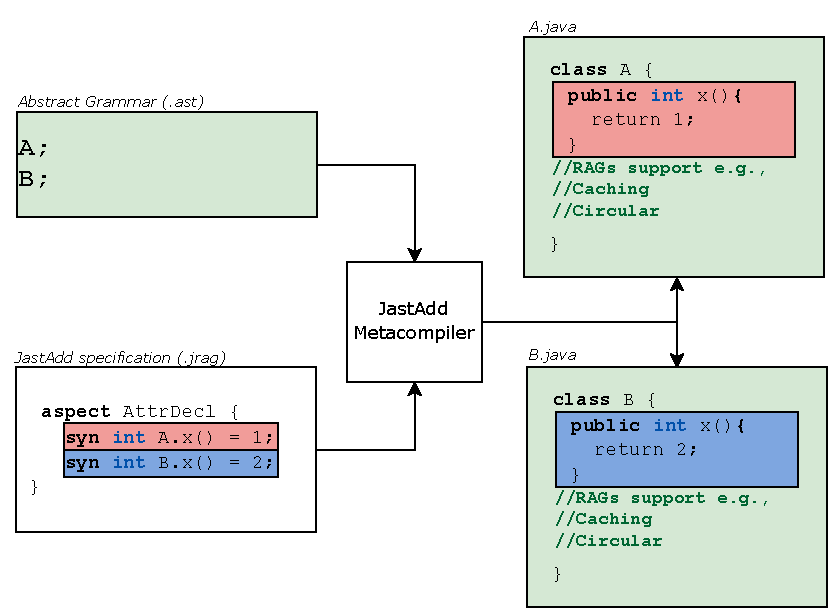
\includegraphics[width=0.85\textwidth]{kappa/img/Intertype.pdf}
  \end{center}
  \caption{\label{fig:interType} \textsc{JastAdd} generates Java classes from the abstract grammar, and
  weaves in code corresponding to the intertype declarations in the aspect into the generated classes \code{A} and \code{B}.
  Additional RAG code for on-demand evaluation support is elided.}
\end{figure}

The example in Figure~\ref{fig:interType}
shows an intertype declaration of an attribute.
The attributes \Asyn{A}{x} and \Asyn{B}{x} are defined in the aspect \code{AttrDecl}
and are woven into the classes \code{A} and \code{B}, respectively.

\textsc{JastAdd} supports not only synthesized and inherited attributes, but also:
\emph{Parametrised Attributes}~\cite{hedin2000rags}, \emph{Higher-Order Attributes}~\cite{vogt1989higher}, \emph{Circular Attributes}~\cite{farrow1986automatic,jones1986hierarchical}, and \emph{Collection Attributes}~\cite{boyland1996descriptional}.


\subsubsection*{Parametrised Attributes} Parametrised Attributes are attributes which value might depend
    not only on the AST node itself, but also on the value of the arguments supplied
    to it. Attributes of this kind are widely used, especially in the definition of
    type-checking rules. For example:
    \begin{lstlisting}[language=JastAdd]
syn boolean Type.compatibleType(Type t) = this == t;
    \end{lstlisting}
    A more advanced set of rules, such as those desigend to handle subtyping,
    would be expected for a real language.
    \subsubsection*{Higher-Order Attribute (HOA)} Higher-Order Attribute, also known as \emph{Non-Terminal Attributes (NTA)}, are attributes which
    value is a freshly new subtree. They are called \emph{Higher-Order Attributes}
    because they are attributes and, at the same time, non-terminal; therefore, they can be attributed.
    The subtree computed by an HOA behaves like a normal AST node, i.e., it can be
    attributed and used in the definition of other attributes. In \textsc{JastAdd}, HOAs
    are defined using the \code{nta} keyword. HOAs are widely used to reify information
    that is not explicit in the source code and, therefore, not present in the AST.
    For example, we use HOAs to reify a method's entry and exit point. In CFGs, it
    is common to have a unique entry point and exit point for each method.
    \begin{lstlisting}[language=JastAdd]
syn nta Entry FunDecl.entry() = new Entry();
syn nta Exit FunDecl.exit() = new Exit();
    \end{lstlisting}
    In our examples, in this thesis, we will often use the right-arrow symbol (\textcolor{ATGsym}{$\rightarrow$}) to
    clarify that an attribute is an HOA. For example, \Ahoa{FunDecl}{entry} and \Ahoa{FunDecl}{exit}.
    %  e.g.,  \Ahoa{FunDecl}{entry} and \Ahoa{FunDecl}{exit}.
    \subsubsection*{Circular Attributes} Circular Attributes are attributes which definition might depend directly
    or indirectly on themselves. In \textsc{JastAdd}, circular attributes are expressed using the \code{circular}
    keyword. To guarantee termination, circular attributes are given a bottom starting value, and are evaluated in a fixed-point
    computation, i.e., the attribute is evaluated until the value of the attribute does not change.
    The requirements, which are not checked by \textsc{JastAdd}, to guarantee termination are:
    \begin{itemize}
        \item All the possible values computed by the attribute must be placed
        in a lattice of finite height.
        \item The intermediate results of the fix-point algorithm must increase
        or decrease monotonically\footnote{In this Thesis, boolean circular attributes start
        as \emph{false} and monotonically grow with $\vee$, while set-typed circular attributes
        start as the empty set and monotonically grow with $\cup$.}.
    \end{itemize}
    We use the symbol \AcircSyn{A}{x} to denote a circular synthesized attribute.
    An example of a circular attribute is the following:
    \begin{lstlisting}[language=JastAdd]
syn int A.x() circular[0] =  Math.min(3, x()+1);
    \end{lstlisting}

In \textsc{JastAdd}, circular attributes are defined using the \code{circular} keyword.
The circular synthesized attribute \AcircSyn{A}{x} begins with a value of 0 and
a fix-point computation is performed until the attribute reaches stability.
In this example, the attribute evaluates to 3 after the third iteration as
the value of the attribute stops changing.

Circular attributes can be used to directly encode mathematical recursive equations,
such as \emph{in} and \emph{out} in the monotone framework.
For example, the equations for the nullness analysis, defined in Section~\ref{sec:dataflowanalysis}, can be written as follows:
\begin{lstlisting}[language=JastAdd, numbers=left]
syn Gamma CFGNode.in() circular[new Gamma()] {
  Gamma res = new Gamma();
  for (CFGNode e : pred())
    res.join(e.out());
  return res;
}

eq Entry.in() = new Gamma(allVars());

syn Gamma CFGNode.out() circular[new Gamma()] {
  Gamma res = new Gamma(in());
  res = trFun(res);
  return res;
}
\end{lstlisting}
The attribute declarations and definitions at Lines 1 and 10, define the $in$ and
$out$ attributes, respectively, for all the CFG nodes.
The attribute equation ad line 8 define the boundary condition for the entry point
of the CFG, i.e., all the variables are mapped to $\bot$.



    \subsubsection*{Collection Attributes}
    Collection Attributes are not defined using equations but instead using the so-called contributions.
    The result of a collection attribute is the aggregation of contributions that can
    come from anywhere in the AST. A contribution clause is associated with
    an AST node type and describes the information to be included in a collection
    attribute, possibly under certain conditions. Collection attributes are especially
    useful, for example, in compiler construction to collect all the semantic errors in a program
    from anywhere in the AST. In \textsc{JastAdd}, collection attributes are defined using the
    \code{coll} keyword.

    An example of a collection attribute is the following:
    \begin{lstlisting}[language=JastAdd]
coll Set<Errors> Program.errors();
Expr contributes this when !type.compatible(expectedType()) to Program.errors();
    \end{lstlisting}
    The collection attribute, \texttt{Program.errors()}, denoted with \Acoll{Program}{errors},
    is used to collect all the semantic errors in the program. The contribution clause
    states that a reference to the \code{Expr} node (i.e., \code{this}) is contributed to the collection when
    the expression type is incompatible with the expected type.
    There can be any number of contribution clauses for a particular collection attribute, so
    new kinds of errors can be added simply by adding new contribution clauses.

    Other examples of using collections include finding reverse relations, for example,
    computing the predecessors in a CFG, given the set of successors.

\subsubsection{Interfaces}
\textsc{JastAdd} supports a mechanism for defining and extending AST classes with interfaces.
Interfaces in \textsc{JastAdd}  provide a way to extend the behaviour
of AST classes. By declaring an interface for an AST class, the class can inherit
equations and attributes defined in the interface.
This enables developers to modularise the behaviour of AST classes, making it easier
to reuse and maintain code.
Interfaces can be declared using the \code{interface} keyword, and, similarly to Java,
they can extend other interfaces.
By using the \code{implements} keyword, it is possible to
state that an AST class implements an interface.
For example, if we want to abstract a common operation for all the CFG nodes, we can define an interface
\astnode{CFGNode} and then specify that all the CFG nodes implement it. For example:
\begin{lstlisting}[language=JastAdd]
public interface CFGNode;

AddExpr implements CFGNode;
AssignStmt implements CFGNode;
//...

syn Gamma CFGNode.in() circular[new Gamma()] {
  Gamma res = new Gamma();
  for (CFGNode e : pred())
    res.join(e.out());
  return res;
}
\end{lstlisting}
In this case, both \astnode{AddExpr} and \astnode{AssignStmt} implement the interface \astnode{CFGNode}.
We then define the \AcircSyn{CFGNode}{in} for the \astnode{CFGNode} interface.
This attribute is then inherited by all the classes that implement the interface,
i.e., \astnode{AddExpr} and \astnode{AssignStmt}, allowing them to share the
common behaviour specified only for \astnode{CFGNode}.
